\subsection{Minimum Bias Event Selection}
The minimum bias event selection criteria are determined using the global detectors: the MBD and ZDC. 
In the MBD, signals are split to read out both the charge and time of each PMT channel. 
Here the charge information relates to the amplitude of the signal waveform and the time information relates to the timing of the waveform peak. 
The timing information has $\sim 50$ ps resolution and is used to calculate the z-vertex of the collision. 
This timing resolution translates to a 1-2 cm resolution in the z-vertex position in minimum bias events that is slightly dependent on the event multiplicity, with high multiplicity events having a smaller z-vertex resolution. 
Additionally, the MBD acts as a multiplicity counter, and therefore, the charge information is calibrated in terms of minimum-ionizing particle (MIP) counts.

Following the MIP counts calibration, loose requirements on individual MBD PMT charge are imposed to classify a PMT as a "fired" tube in the MBD and for that charge information to be included in the total MBD charge sum used for centrality calibration.
These MBD PMT hit requirements are $q > 0.5$ in MIP counts and a time between $-20 < t < 20$ ns. 
Figure~\ref{fig:mbd_pmt_hit_criteria} shows the full PMT charge and time distributions for an example PMT with the hit requirement cuts overlaid. 
The PMT MIP peak is clearly visible in the charge distribution and $q > 0.5$ is well below the MIP peak. 
Additionally, the loose timing cuts applied are well outside the main collision timing distribution.

\begin{figure}
    \centering
    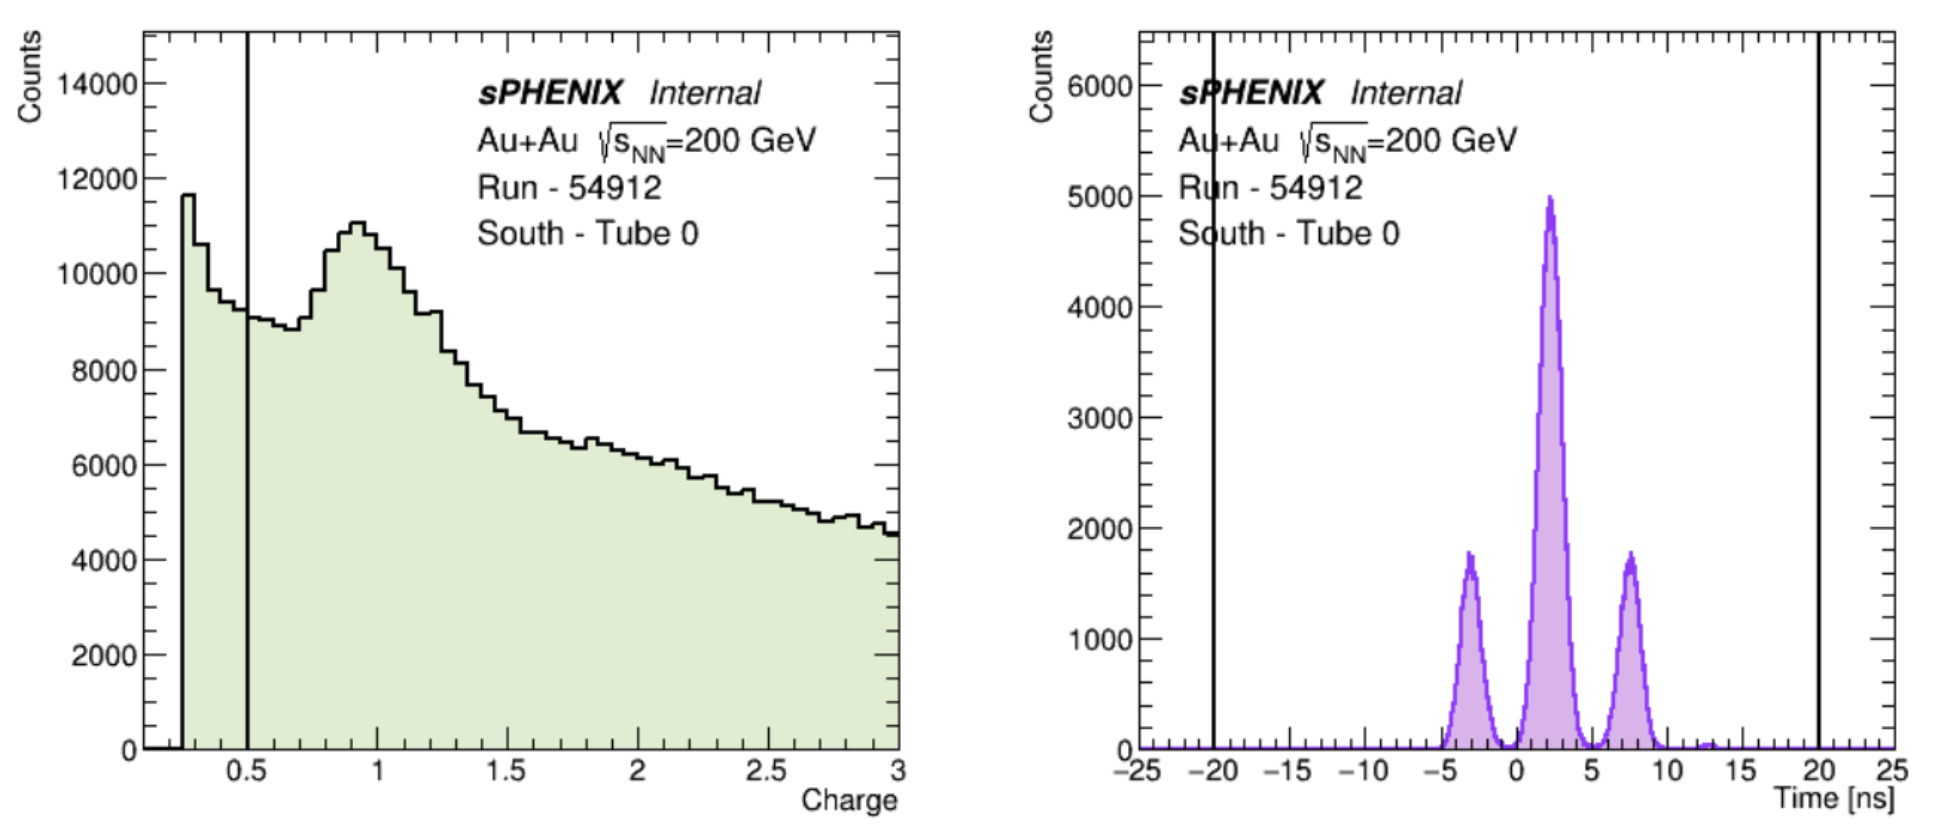
\includegraphics[width=\linewidth]{figures/chapter4/mbd_hit_criteria_centrality_note.png}
    \caption{MBD PMT charge (left) and time (right) distributions for example individual PMT with PMT hit requirements ($q > 0.5$ and $-20 < t < 20$ ns) included (black lines). Time distribution has three peaks corresponding to the main collision bunch around 2 ns and satellite bunches around -3 and 7 ns. Reproduced from \cite{Lis1}.}
    \label{fig:mbd_pmt_hit_criteria}
\end{figure}

Events in both data and MC are selected using the following minimum-bias event selection criteria in order to ensure high purity and efficiency of hadronic collisions in the minimum bias dataset \cite{Lis1}. 
The selection requirements are as follows: 
\begin{itemize}
    \item MBD $\textit{N}_{\textit{tubes,N}} \geq 2 \, \& \, \textit{N}_{\textit{tubes,S}} \geq 2$ 
    \item $\Sigma Q_{MBD,N} > 10 \lor \Sigma Q_{MBD,S} < 150 $
    \item $\Sigma E_{ZDC,N} > 40\, \text{GeV}\, \& \, \Sigma E_{ZDC,S} > 40\, \text{GeV} $
    \item $\mid z_{vtx,MBD}\mid < 60$ cm
\end{itemize}

The first requirement is the hardware level MBD trigger requirement. 
This requirement is also required in the offline reconstruction since online and offline MBD charge calibration factors can be slightly different.
The second requirement removes nonphysical backgrounds in the MBD charge distribution determined from studies of the charge correlation between the two sides of the MBD. 
Figure~\ref{fig:mbd_ns_correlation} shows the region of nonphysical background events removed using this second requirement on the MBD charge sum. A large fraction of these nonphysical background events are from material upstream in the beamline which results in an asymmetric effect on the MBD charge sum correlation between the two sides of the MBD. 
The third requirement is a requirement of energy in both sides of the ZDC to remove any remaining beam backgrounds that may still pass the hardware trigger from the MBD, like beam-gas interactions.
An energy requirement of 40 GeV is used for the ZDC hit requirement since the ZDC response to spectator neutrons is fully efficient at 40 GeV when the ZDC is calibrated so that the single spectator neutron peak is at 100 GeV.
Figure~\ref{fig:zdc_efficiency_run_by_run} shows the run dependence of including this ZDC requirement in the minimum bias criteria.
Here there is a small store dependence, where a store contains consecutive runs all within one fill of the RHIC ring with ions, with more significant beam losses at the start of a store than later in the store; 
this higher rate of beam backgrounds at the start of a store can be seen in the lower ZDC hit efficiency in the minimum bias definition at the start of the store which then levels off later in the store as background rates are lower. 
Later in the store there still remains a 2\% difference in the minimum bias definition with and without the ZDC requirement which can be due to very peripheral events only having a spectator neutron on one side or the other. 
Due to modeling limitations in simulation, the ZDC requirement is not included in the selection requirements in simulation.
Therefore, this 2\% difference in the minimum bias definition from this ZDC requirement is included as a 2\% uncertainty downwards on the minimum bias trigger efficiency.

\begin{figure}
    \centering
    \begin{subfigure}{0.65\linewidth}
        \centering
        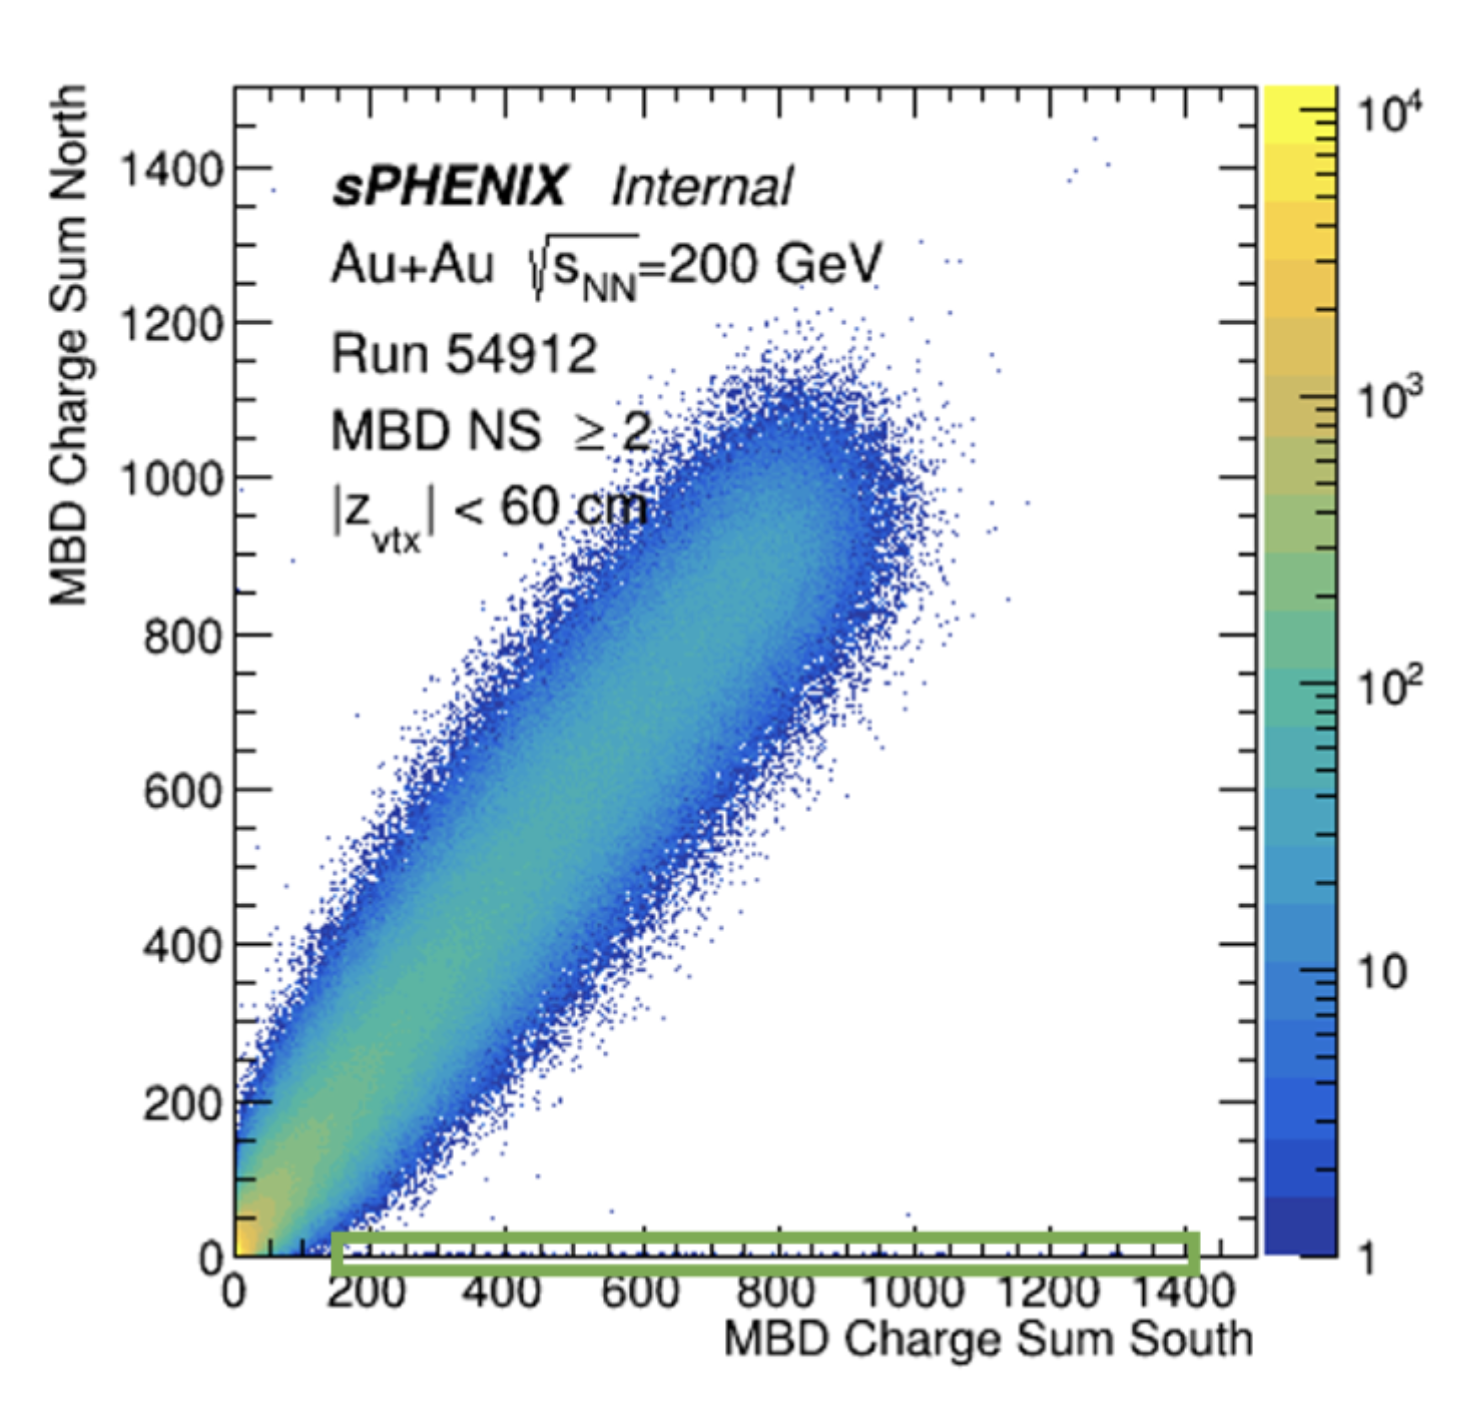
\includegraphics[width=\linewidth]{figures/chapter4/mbd_correlation_centrality_note.png}
        \caption{MBD Charge Sum Correlation of North and South Sides}
        \label{fig:mbd_ns_correlation}
    \end{subfigure}
    \hfill
    \begin{subfigure}{0.65\linewidth}
        \centering
        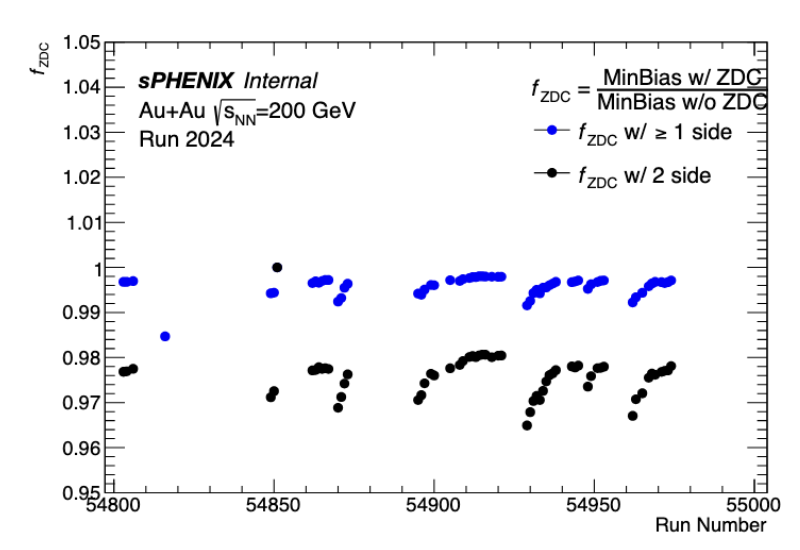
\includegraphics[width=\linewidth]{figures/chapter4/zdc_efficiency_centrality_note.png}
        \caption{Run Dependent ZDC Hit Efficiency}
        \label{fig:zdc_efficiency_run_by_run}
    \end{subfigure}
    \caption{(a) Correlation between the charge sum on two sides of the MBD (North and South). Green rectangle shows region of nonphysical background events removed by second MB requirement. (b) Run dependence of the efficiency of a ZDC hit in one (blue points) or both (black points) sides of the ZDC in MBD-determined minimum bias events. Reproduced from \cite{Lis1}.}
\end{figure}

Figure~\ref{fig:mbd_zdc_correlation} shows the correlation between the energy in the ZDC and MBD charge sum for events passing these minimum bias event selection criteria.
A characteristic decrease in the total ZDC energy is observed at both high and low MBD charge. 
This corresponds to regions of very central collisions, where only a small number of spectator neutrons deposit energy in the ZDC, and to peripheral collisions, where most spectator neutrons are bound in larger charged nuclear fragments deflected away from the ZDC by the RHIC magnets, respectively.
Finally, for the \detdeta measurement, a tighter cut has been applied on the z-vertex, $\mid z_{vtx,MBD} \mid < 10$ cm, since the calorimeter towers are projective in $\eta$ from the nominal center of the detector at z = 0. 
This tighter z-vertex cut is also applied to avoid large fluctuations in the calorimeter acceptance region of $\eta$ < 1.1 as a result of a wide collision vertex distribution.
Events were further selected to be in the centrality range of 0-70\% to ensure complete minimum-bias event selection efficiency, while also including a broad range of geometric sizes of the produced QGP. 
Combining all these selections, the total number of events used in the \detdeta measurements of events with centrality between 0 and 70\% corresponds to 518,000 events.

\begin{figure}
    \centering
    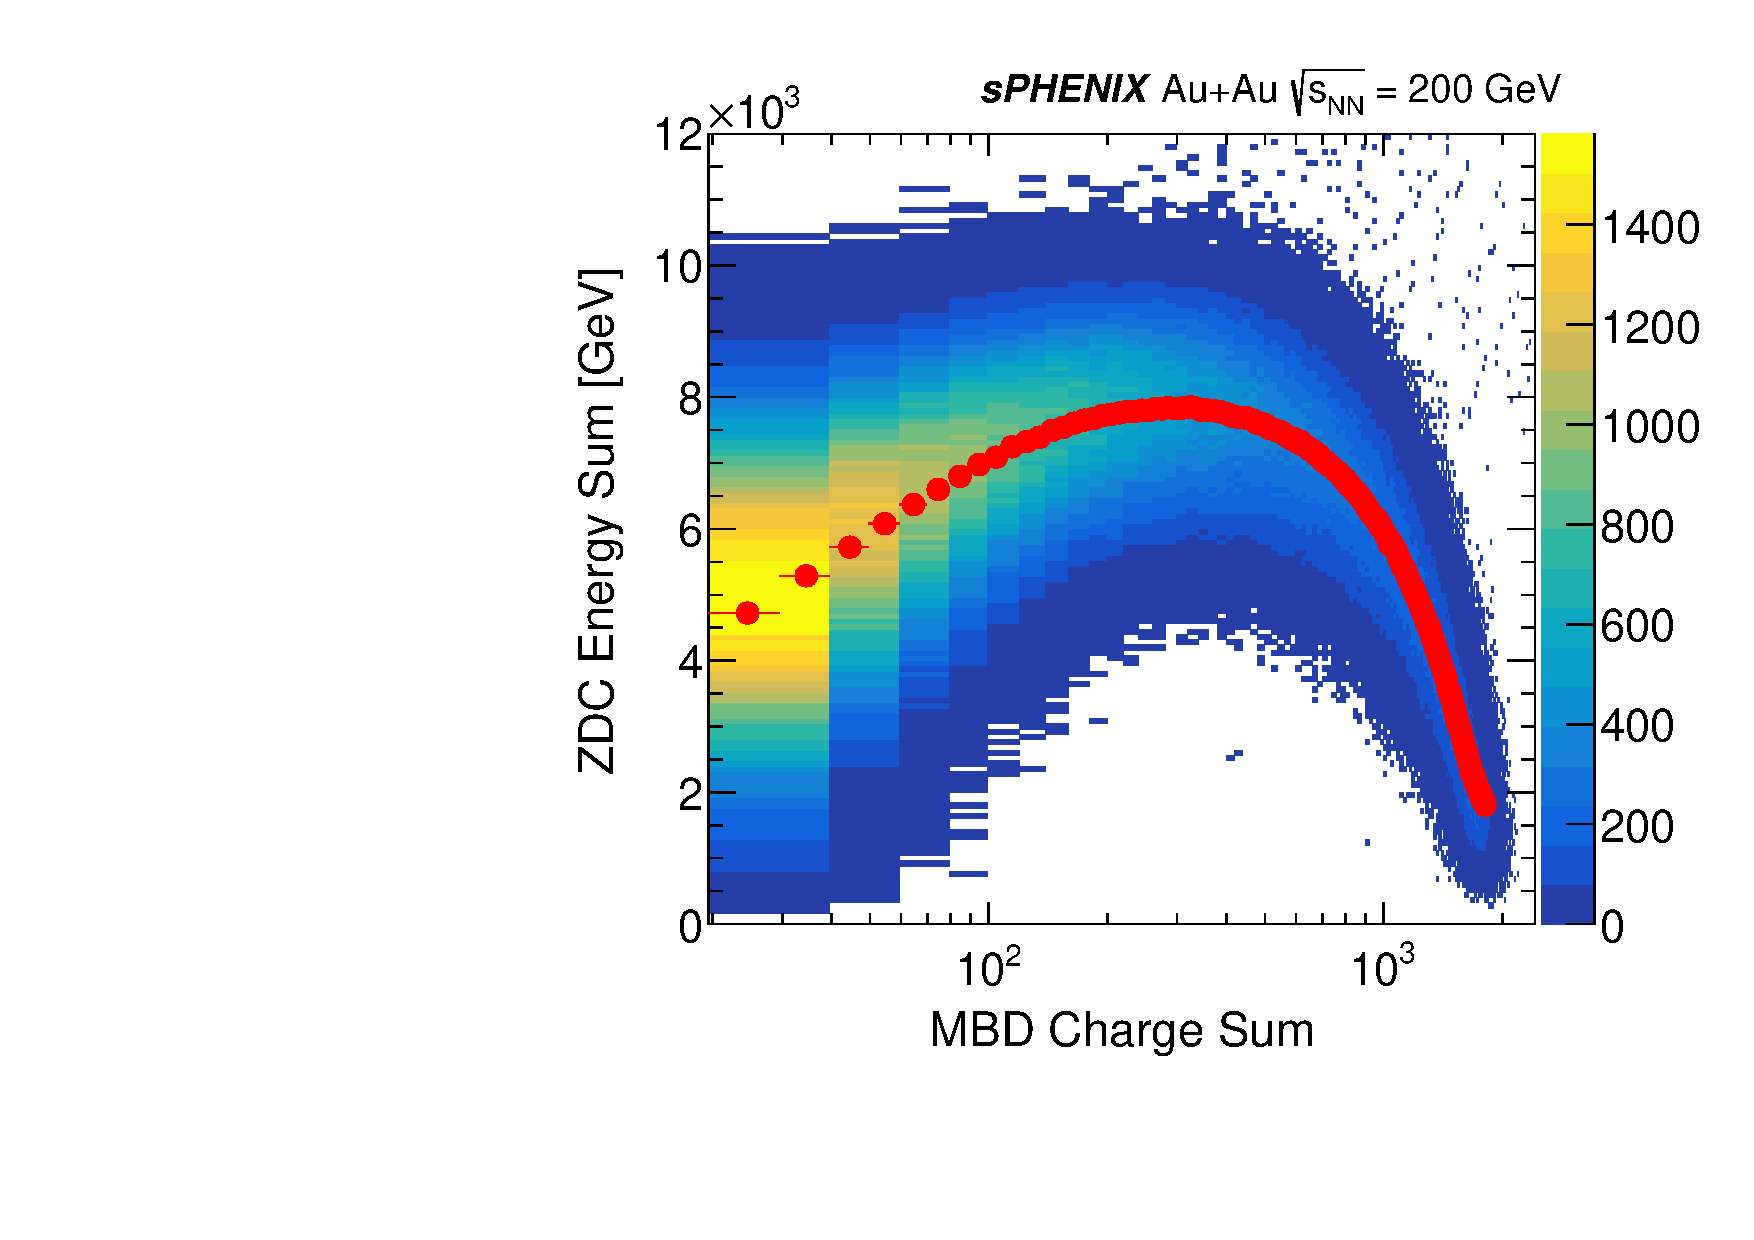
\includegraphics[width=0.9\linewidth]{figures/chapter4/run54912_charge_sum_zdc.pdf}
    \caption{The correlation between the total energy in ZDCs and the MBD charge sum is shown. The MBD charge sum is in units of calibrated MIPs. The red points indicate the average ZDC energy as a function of MBD charge sum. Reproduced from \cite{sphenix_detdeta}}
    \label{fig:mbd_zdc_correlation}
\end{figure}

\subsection{Event Centrality Determination}
Events in both data and MC are assigned a centrality value which characterizes the level of geometric overlap between the two colliding nuclei.
The MBD charge sum distribution for all events passing the minimum bias event selection is fit to the MC Glauber $\oplus$ Negative Binomial Distribution (MBD) model.
The first part of this model is a MC Glauber simulation, which simulates the nuclear geometry event-by-event and outputs nuclear geometry information such as the impact parameter, b, number of participating nucleons, $\Npart$, and number of nucleon collisions, $\Ncoll$.
The second part of the model uses a negative binomial distribution to get a realistic distribution of the final state multiplicity by finding the mean and width of the NBD distribution needed to have the $\Npart$ distribution from the MC Glauber model match the MBD charge distribution in data.
For this analysis, the best matched NBD parameters are found to be $\mu = 4.74$ and $k = 1.17$~\cite{Lis1}.

The MC Glauber nucleon-nucleon cross-section, nuclear radius, and Woods-Saxon skin thickness parameters are given in Table \ref{tab:glauber} and the MC Glauber $\oplus$ NBD result is fit to the MBD charge sum distribution for the minimum bias trigger's fully efficient region ($\Sigma Q_{MBD} > 150 N_{MIP}$) to determine the best parameter values for the NBD. 
The MBD charge sum distribution with fit to the MC Glauber $\oplus$ NBD model is shown in Figure~\ref{fig:mbd_charge_sum}.
By extracting the integral of the MBD charge sum distribution and fitted MC Glauber $\oplus$ NBD result, the minimum bias event selection efficiency was determined to be $93.4\%^{+3.4\%}_{-3.1\%}$ of the Au+Au inelastic cross section and centrality intervals are determined as percentiles of the minimum bias event distribution between 0 and 93\%. 
The bottom panel of Figure~\ref{fig:mbd_charge_sum} shows the peripheral event region in detail to highlight this minimum bias trigger efficiency turn-on region. 
The resulting Glauber parameters and extracted $\Npart$ values for each centrality interval are included in Table~\ref{tab:glauber}.
Figure~\ref{fig:npart_ncoll_b} also includes a reference of the relationship between $\langle \Npart \rangle$, $\langle \Ncoll \rangle$ and the collision impact parameter, b, to highlight the range in nuclei-nuclei geometric overlap in this analysis.

\begin{figure}
    \centering
    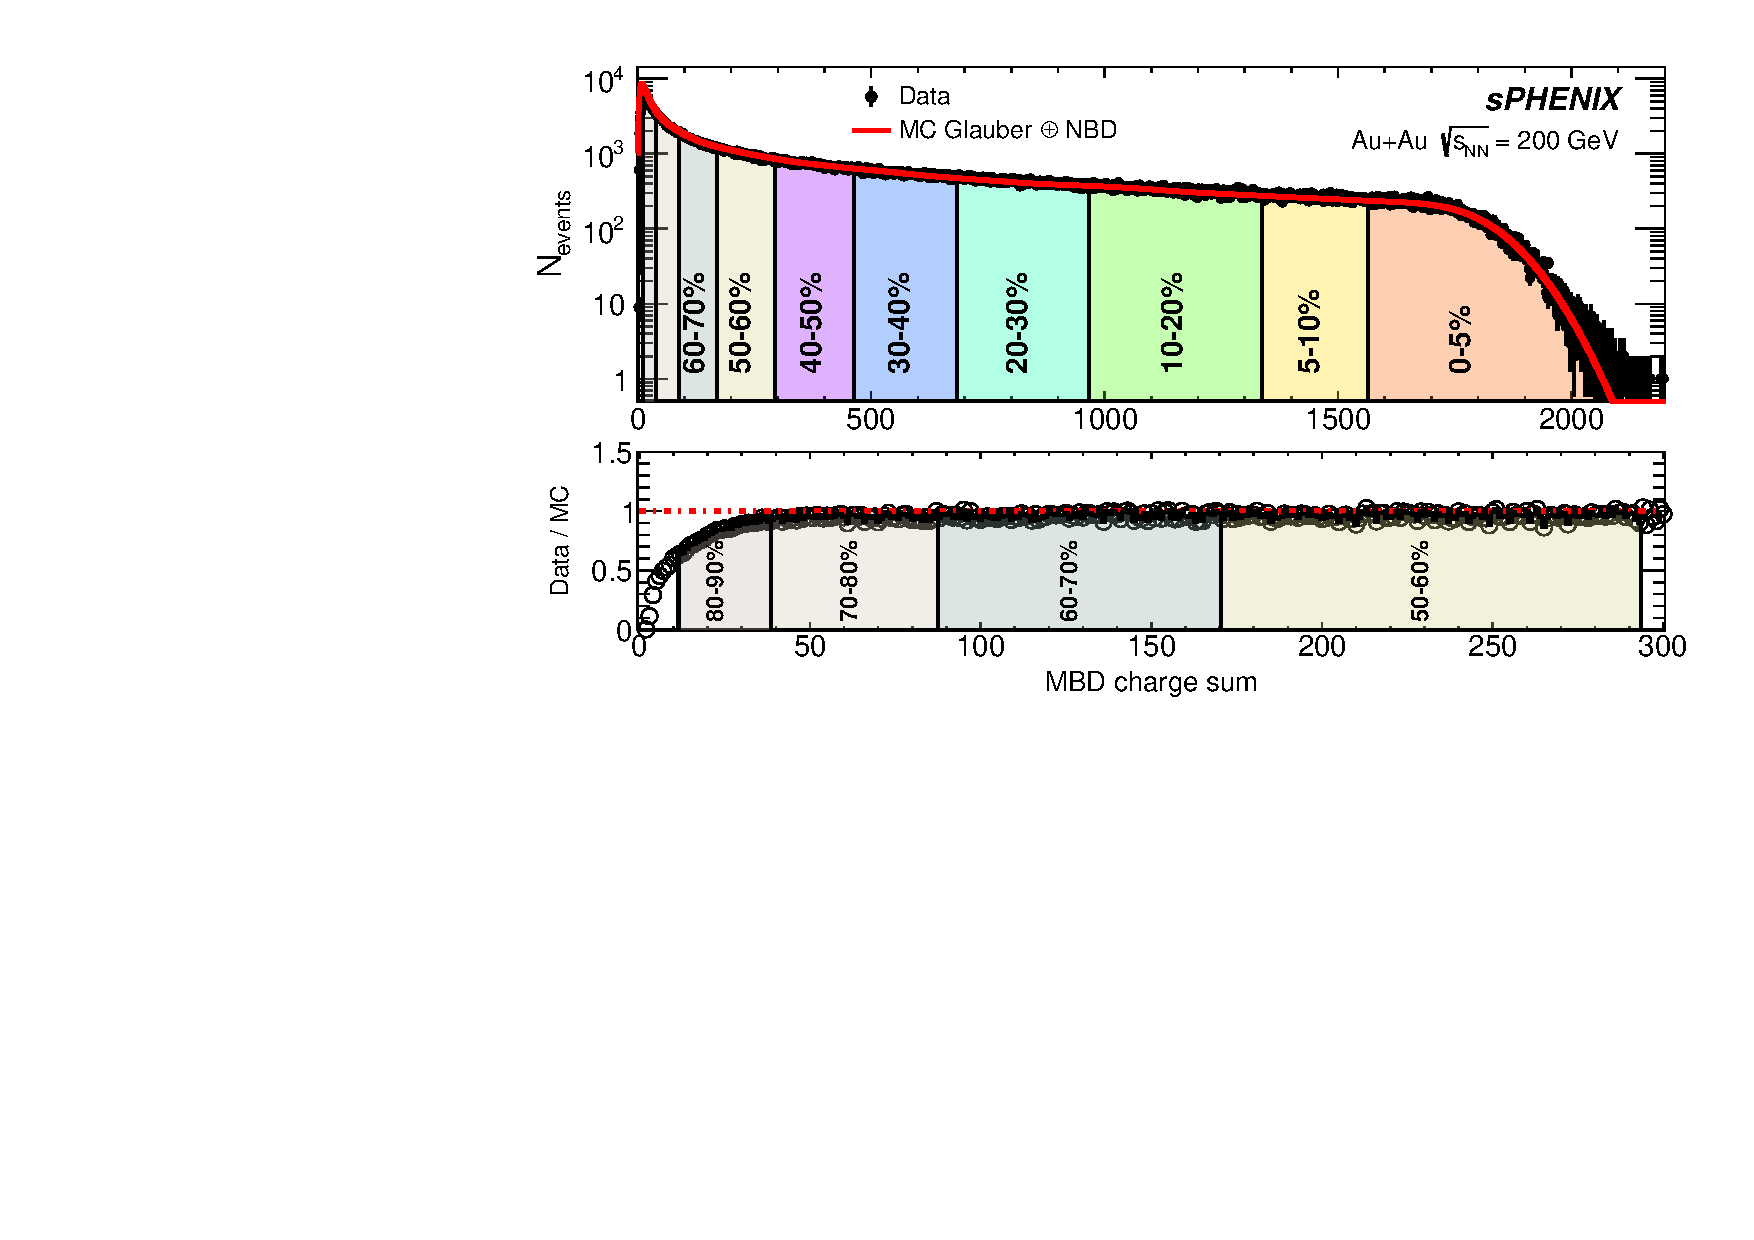
\includegraphics[width=\linewidth]{figures/chapter4/PPG03_Fig1_updated_20250728.pdf}
    \caption{The MBD charge sum distribution in minimum-bias Au+Au events (points), compared to the best fit from a MC Glauber $\oplus$ NBD simulation (red line). The shaded bands indicate 5-10\% wide centrality intervals. The lower panel highlights the ratio of the MBD charge sum to the MC Glauber $\oplus$ NBD fit in the peripheral event region, showing the effect of the trigger turn-on. The MBD charge sum is in units of calibrated MIPs. Reproduced from \cite{sphenix_detdeta}.}
    \label{fig:mbd_charge_sum}
\end{figure}

\begin{table}
\begin{subfigure}[t]{0.45\textwidth}
\centering
    \renewcommand{\arraystretch}{1.5}
    \begin{tabular}{cc}
    Glauber Parameter & Value \\
    \hline
    $\sigma_{NN}$ [mb] & $42 \pm 3$ \\
    Nuclear radius [fm] & $6.38_{-0.13}^{+0.27}$ \\
    Skin depth [fm]  & $0.535_{-0.010}^{+0.020}$ 
    \end{tabular}
\end{subfigure}
\begin{subfigure}[t]{0.45\textwidth}
\centering
    \renewcommand{\arraystretch}{1.3}
 \begin{tabular}{cc}
    Centrality interval & \Npart \\
    \hline
        0-5\% & $350.0 \pm 2.2$ \\
        5-10\% & $301.8 \pm 3.2$ \\
        10-20\% & $238.1 \pm 4.1$ \\
        20-30\% & $170.8 \pm 4.9$ \\
        30-40\% & $118.5 \pm 5.2$ \\
        40-50\% & $78.3 \pm 5.1$ \\
        50-60\% & $47.8 \pm 4.5$ \\
        60-70\% & $26.1 \pm 3.6$ \\
    \end{tabular}
\end{subfigure}
\caption{Glauber model parameters (left) for \auau{} collisions at \sqsntwo. Centrality intervals and average number of participating nucleons ($\Npart$) for \auau collisions at \sqsntwo (right) obtained using Glauber model. Reproduced from \cite{sphenix_detdeta}.}
\label{tab:glauber}
\end{table}

\begin{figure}
    \centering
    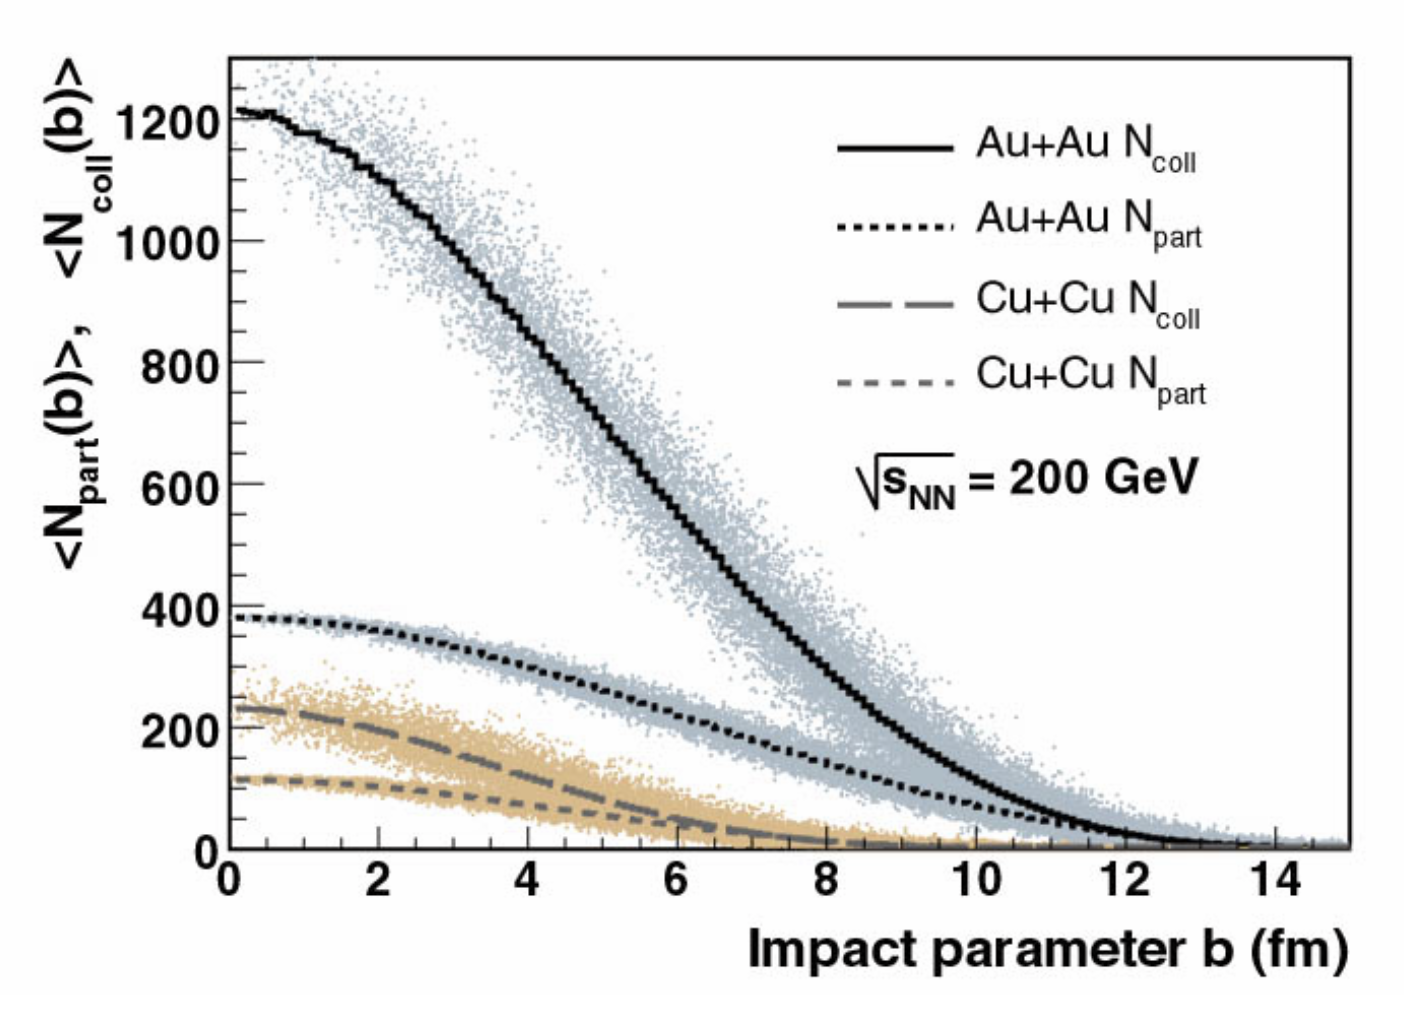
\includegraphics[width=0.7\linewidth]{figures/chapter4/npart_ncoll_vs_b}
    \caption{Distributions of $\langle \Npart \rangle$ and $\langle \Ncoll \rangle$ as a function of impact parameter for Cu+Cu (brown) and Au+Au (gray) collisions at $\sqsntwo$. Mean values are included as lines and event-by-event fluctuations are included as scatter points. Reproduced from \cite{glauber_review}.}
    \label{fig:npart_ncoll_b}
\end{figure}

\subsection{Centrality Determination in MC}

A minimum bias event selection and centrality percentile determination was also performed on the three MC datasets: \hijing, \ampt and \epos events passed through the \geant simulation.
The same MC Glauber $\oplus$ NBD fitting procedure is carried out in simulation, here based on the simulated MBD PMT hits and total charge sum distribution, providing event-by-event centrality characterization in the same way as in data~\cite{Lis1}. 

Additionally, in simulation the efficiency of the minimum bias trigger requirement was also studied. 
A consistent 3\% discrepancy was found for all three generators between the trigger efficiency extracted from the MC Glauber $\oplus$ NBD fitting to the simulated MBD charge sum distribution and the fraction of generated minimum bias events that pass the minimum bias trigger requirement.
This discrepancy is also included in the systematic uncertainty on the minimum bias trigger efficiency. 